% UTF-8

% single-chapter commands
\documentclass[../main/thesis.tex]{subfiles}
\onlyinsubfile{\setcounter{chapter}{5}}  % single-chapter command
\begin{document}


\chapter{Ergebnisdiskussion}
% Beschreibung, was tatsächlich die Software ausspuckt, wo's hakt und wo ich noch gebastelt habe
% alles NUR im "Anwendungskontext", d.h. in Bezug auf die Ausgabe-Geodaten, nicht die Softwarequalität (das war in 5.4!)
% Schritt für Schritt Probleme sammeln und katalogisieren

%Die in Kap. 4 und 5 entwickelte Software ist das Ergebnis dieser Arbeit. Hier diskutiert werden soll die Arbeitsweise dieser Software und die Qualität der von ihr ausgegebenen Geodaten in Bezug auf die Aufgabenstellung.

Bei der Evaluierung der Software ist zu bedenken, dass die \osm-Datenbank ständig bearbeitet wird.
Konsistente Ergebnisse für ein bestimmtes Gebiet erfordern daher, dass immer mit Geodaten vom selben Stand gearbeitet wird.
Soweit nicht anders angegeben, beschränkt sich dieses Kapitel auf einen Datensatz mit dem Straßennetz im Land Nordrhein-Westfalen vom November~2012.
% http://dev.thaw.de/temp/highways/nrw-roads.zip (testbed-nrw-prepare.sh)

% möglichst auch Untersuchung der Anwendung des Algorithmus auf Straßen in unterschiedlichen Regionen der Welt



\section{Anwendung in einfachen Situationen}

Bei Anwendung der mit dieser Arbeit entwickelten Software auf Geodaten aus der \osm-Datenbank zeigt sich, dass die implementierten Algorithmen grundsätzlich funktionieren.

\onefigure{p}{
	\twofigures{H}{
		\begin{overpic}[width=\ScaleIfNeeded]{../chapter6/result-trivial-in}
			\put(122,84){\figuremark{1}}
			\put(58,60){\figuremark{2}}
			\put(23,39){\rotatebox{50}{\figureframe{.1167}}}
		\end{overpic}
	}{
		\begin{overpic}[width=\ScaleIfNeeded]{../chapter6/result-trivial-out}
			\put(122,84){\figuremark{1}}
			\put(58,60){\figuremark{2}}
			\put(23,39){\rotatebox{50}{\figureframe{.1167}}}
		\end{overpic}
	}
	% trivial = testbed-nrw/koeln-classfied-nolinks.shp
	% 1:30000 Google Mercator, bbox 778765 6607045 780865 6608245, 0.2mm stroke
	\caption{Ergebnis der Software im einfachen Fall (links Eingangsdaten, rechts Generalisierungsergebnis; Köln-Gremberg mit Autobahn L\,124)}
	\label{fig:result-trivial}
}

In Abbildung~\ref{fig:result-trivial} sind links \osm-Linienzüge in der einfachen Situation einer Autobahn ohne Anschlussstellen nebst innerstädtischen Sammelstraßen zu sehen.
Durch Anwendung der Software ergibt sich das rechts dargestellte automatisiert zusammengefasste Ergebnis.
Anstelle der beiden Richtungsfahrbahnen der Autobahn gibt es nun nur noch einen einzigen Linienzug als Straßenachse.
Die Nähe zu nachgeordneten Straßen und deren planfreie Kreuzung mit der Autobahn (bei Markierung~\textfiguremark{1}) stört die Generalisierung nicht.
Auch eine Strecke paralleler Fahrbahnen im nachgeordneten Netz wurde trotz eines scharfen Knicks erfolgreich als parallel erkannt und zusammengefasst (Markierung~\textfiguremark{2}).

Abbildung~\ref{fig:result-trivial-styled} zeigt beispielhaft, wie sich dieses Generalisierungsergebnis sinnvoll visualisieren ließe.
Die Software kennzeichnet die zusammengefassten Linienzüge als generalisiert.
Zusätzlich gibt die Software einzelne \term{tags} der \osm-Quelldaten mit aus.
Anhand dieser Attribute können leicht Regeln mit jeweils passenden Linearsignaturen definiert werden.

\onefigure{p}{
	\twofigures{H}{
		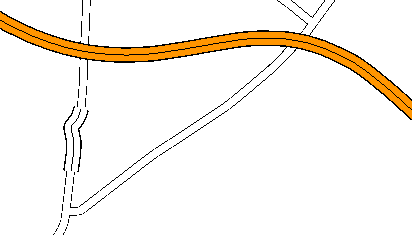
\includegraphics[width=\ScaleIfNeeded]{../chapter6/result-trivial-styled}
	}{
		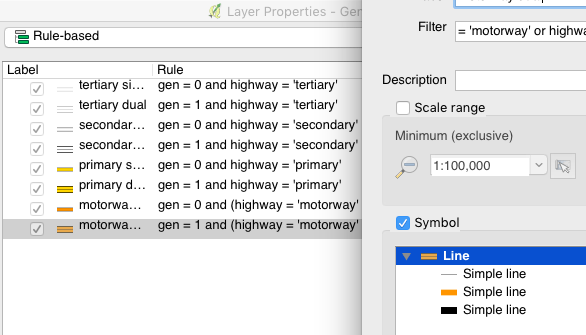
\includegraphics[width=\ScaleIfNeeded]{../chapter6/result-trivial-rules}
	}
	\caption{Visualisierung des Generalisierungsergebnisses (links Kartendarstellung, rechts Screenshot der Zeichenregeln in QGIS)}
	\label{fig:result-trivial-styled}
}

Bei näherer Betrachtung ist die korrekte Arbeitsweise der implementierten Algorithmen in diesem einfachen Fall gut zu erkennen (Abbildung~\ref{fig:result-trivial-detail-rolshover}):
Linienzüge werden durch \textproc{Splitten} derart unterteilt, dass möglichst jeweils zwei Punkte auf Parallelen einander gegenüber liegen (gut zu sehen bei Markierung~\textfiguremark{1}).
Die dabei entstehenden einander gegenüberliegenden Fragmente sind durch ihre Ähnlichkeit offensichtlich einfach auf Parallelität zu prüfen.
Selbst dann, wenn beim \textproc{Splitten} keine optimalen Paare entstehen, gelingt dies, solange wenigstens jeweils ein \emph{Teil} der miteinander verglichenen Segmente zueinander parallel ist (\textfiguremark{2}).
Von diesen Zuordnungen der einander gegenüberliegenden \osm-\term{nodes} lässt sich durch Verbindung ihrer Mittelpunkte leicht eine Mittellinie im Verlauf der Straßenachse als Ergebnis ableiten.

% writeNodeMatches
\onefigure{p}{
	\twofigures{H}{
		\begin{overpic}[width=\ScaleIfNeeded]{../chapter6/result-trivial-detail-rolshover}
			\put(129,0){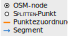
\includegraphics{../chapter6/legend-nodematch}}
			\put(53,7){\figuremark{1}}
			\put(95,51){\figuremark{2}}
			\put(184,83){\figuremark{3}}
		\end{overpic}
	}{
		\begin{overpic}[width=\ScaleIfNeeded]{../chapter6/result-trivial-detail-rolshover-gen}
			\put(129,0){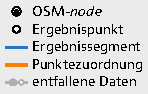
\includegraphics{../chapter6/legend-nodematch-gen}}
			\put(53,7){\figuremark{1}}
			\put(88,44){\figuremark{2}}
			\put(184,83){\figuremark{3}}
		\end{overpic}
	}
	% 1:3500 Google Mercator rotated 50°, bbox 779025 6607525 779270 6607665
	\caption{Detaildarstellung Generalisierung mit Punktezuordnungen (links Eingangsdaten, rechts Generalisierungsergebnis; \textfiguremark{2}~in Abbildung~\ref{fig:result-trivial})}
	\label{fig:result-trivial-detail-rolshover}
}

Der Übergang zwischen generalisierten und nicht generalisierten Linienzügen (\textfiguremark{3}) wird unten im Abschnitt~\ref{ch:relocateGeneralisedNodes} diskutiert.

Für den NRW-Testdatensatz wurden die in Abschnitt~\ref{ch:analyse-algorithm} genannten Beispielwerte von höchstens um $15\degree$ abweichender Ausrichtung und höchstens $\unit[40]{m}$ Abstand zweier \textproc{Parallel}er Segmente empirisch als grundsätzlich tauglich bestätigt.
% evtl. näher ausführen, Tabelle mit Zahlen machen, ...
Für Autobahnen genügt überwiegend bereits ein Limit von nur $10\degree$ Abweichung.
Sonstige Straßen besitzen wesentlich engere Kurvenradien und haben vereinzelt Segmente, welche als parallel gelten könnten, deren Ausrichtung jedoch um $30\degree$ oder mehr voneinander abweicht.

% Ausrichtungsgrenze 15°:
% - empirisch ermittelter vernünftiger Bereich für autobahnähnlich etwa 8..16°
% - empirisch ermittelter vernünftiger Bereich für innerstädtisch etwa 20..40°

% Distanz 40 m:
% - empirisch ermittelter vernünftiger Bereich für autobahnähnlich etwa 40..45 m
% - empirisch ermittelter vernünftiger Bereich für innerstädtisch etwa 35..50 m

Um Praxistauglichkeit zu erreichen, müsste die Definition von \textproc{Parallel} folglich vom Straßentyp abhängen.
Dies wurde aus Zeitgründen nicht mehr als Teil dieser Arbeit umgesetzt.

Der NRW-Testdatensatz enthält als \osmtag{highway}[motorway] attributierte Linienzüge mit einer Gesamtlänge von $\unit[4515]{km}$.
% roads-motorway.shp
Die entwickelte Software erkennt $\unit[4461]{km}$ davon als parallel; das ausgegebene Ergebnis besteht zu $\unit[97,6]{\%}$ aus zusammengefassten Linienzügen.
Nachdem alle nordrhein-westfälischen Autobahnen zweibahnig ausgebaut sind, wäre bei naiver Betrachtung eine Erkennungsrate von $\unit[100]{\%}$ zu erwarten gewesen.
Die Untersuchung der ausgegebenen Ergebnisdaten hat gezeigt, dass Linienzüge im Wesentlichen in den folgenden Fällen als \emph{nicht} parallel erkannt werden:

\begin{itemize}[nosep]
\item fehlerhafte Klassifizierung (\osmtag{highway}) von Auf- und Abfahrten
% (insb. \osmtag{highway}[motorway] statt \term{motorway\_link})
\item fehlerhaftes Attribut für die Straßennummer (\osmtag{ref})
% \osmtag{ref} einseitig fehlend oder voneinander abweichend
\item definierte geometrische Kriterien für Parallelität sind nicht erfüllt \\(z.~B. ungewöhnlich großer Abstand der Richtungsfahrbahnen)
\end{itemize}
%
Letzteres ist zu erwarten und offensichtlich korrekt.
Die ersten beiden Fälle werden in den folgenden Abschnitten~\ref{ch:result-tags} und~\ref{ch:result-junctions} näher betrachtet.



\section{Berücksichtigung von Attributen}
\label{ch:result-tags}

Die in Abschnitt~\ref{ch:analyse-algorithm} beschriebenen Algorithmen berücksichtigen neben der Klassifizierung der Straße als einziges Attribut die Straßennummer.
% in der Annahme, dass diese normalerweise stimmt
Im NRW-Testdatensatz erkennt die Software $\unit[54]{km}$ Fahrbahn nicht als parallel; wird die Straßennummer nicht berücksichtigt, sinkt diese Länge auf $\unit[31]{km}$.

An mehreren der dann neu erkannten Stellen trägt nur eine der beiden Richtungsfahrbahn die Straßennummer als Attribut.
Entgegen der Annahme in \label{ch:case-selection} fällt dies den \osm-Beitragenden beim Betrachten von Karten nicht unbedingt auf, solange die Straßennummer der \emph{anderen} Richtungsfahrbahn korrekt angezeigt wird.

Vereinzelt existieren auch widersprüchliche Straßennummern der beiden Richtungsfahrbahnen.
So ist auf mehreren Abschnitten bei Dülmen die eine Fahrbahn \osmtag{ref}[A\,43] gekennzeichnet, die andere jedoch \osmtag{ref}[A\,43;B\,474], während bei Bliesheim eine der Richtungsfahrbahnen der A\,553 das Attribut \osmtag{ref}[A\,1] trägt.

Da in diesen Fällen die Geometrie der Fahrbahnen offensichtlich parallel ist, muss hinterfragt werden, welche Bedeutung den Attributen beigemessen werden sollte.
%
% für Kap. 7:
%Statt eines harten Ausschlusskriteriums wie in Abschnitt~\ref{ch:analyse-algorithm} definiert scheint es sich anbieten, aus der Geometrie und den Attributen eine \emph{Wahrscheinlichkeit} abzuleiten, mit der die verglichenen Segmente insgesamt parallel sind, und als einziges \emph{hartes} Kriterium einen Schwellenwert für diese Wahrscheinlichkeit vorzusehen.
%Es könnten dann auch leicht weitere Attribute wie Straßenname oder die vertikale Ebene in angemessenem Umfang berücksichtigt werden, ohne dass einzelne Aspekte, die falsch attribuiert sind, ein korrektes Ergebnis verhindern.
%Diese Idee wurde aus Zeitgründen nicht mehr als Teil dieser Arbeit umgesetzt.
%
Die entwickelte Software berücksichtigt derzeit entgegen der ursprünglichen Definition standardmäßig nicht mehr die Straßennummer.
%Auch dies könnte jedoch zu Problemen führen, weil damit zwei Fahrbahnen gleicher Klassifizierung, die nur zufällig parallel sind, jedoch zu unterschiedlichen Straßen gehören, fälschlich als Richtungsfahrbahnen derselben Straße erkannt werden könnten.
Dieses Verhalten kann mit dem Schalter \texttt{--tags} kontrolliert werden.



\section{Verhalten an Straßenkreuzungen}
\label{ch:result-junctions}

\subsection{Beseitigung von Topologielücken}
\label{ch:relocateGeneralisedNodes}

Beim Zusammenfassen von Linienzügen erzeugt die Software neue Stützpunkte entlang einer Mittellinie.
Werden die Stützpunkte der ursprünglichen Linienzüge noch für weitere Zwecke verwendet, dürfen diese nicht entfallen, sondern müssen erhalten bleiben.

An \term{nodes}, die sowohl beim Zusammenfassen entfallene Linien als auch andere Linien benutzen, wird dies zum Problem:
Sie werden von nicht generalisierten Linien weiterbenutzt, die generalisierten Linien hingegen verwenden die neu erzeugten Punkte, so dass an den Übergängen topologische Lücken im Straßennetz entstehen.
Die entwickelte Software versucht dem zu begegnen, indem die \term{nodes} an den Enden \emph{nicht} generalisierter Linienzüge auf diese Situation hin geprüft und nötigenfalls durch geeignete Punkte auf der generalisierten Mittellinie ersetzt werden.

\onefigure{h}{
	\twofigures{H}{
		\begin{overpic}[width=\ScaleIfNeeded]{../chapter6/koelnarena-gen}
			\put(0,0){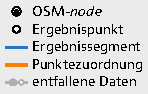
\includegraphics{../chapter6/legend-nodematch-gen}}
			\put(51,67){\figuremark{1}}
			\put(137,24){\figuremark{2}}
		\end{overpic}
	}{
		\begin{overpic}[width=\ScaleIfNeeded]{../chapter6/koelnarena-gen-cleanup}
			\put(0,0){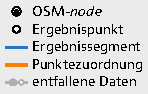
\includegraphics{../chapter6/legend-nodematch-gen}}
			\put(51,67){\figuremark{1}}
			\put(137,24){\figuremark{2}}
		\end{overpic}
	}
	% 1:5500 Google Mercator, bbox 777275 6610050 777660 6610270
	\caption{Detaildarstellung der Beseitigung von Topologielücken (links vorher, rechts nachher; L\,111 in Köln-Deutz)}
	\label{fig:koelnarena-gen-cleanup}
}

Abbildung~\ref{fig:koelnarena-gen-cleanup} zeigt, dass diese Lösung grundsätzlich funktioniert.
Die Straßenkreuzung bei \textfiguremark{1} wird auf einen einzelnen Punkt zusammengefasst, so dass beide Straßen korrekt miteinander verknüpft sind.
Auch der bereits in Abschnitt~\ref{ch:generalisation-algorithm} angesprochene und zunächst offen gelassene Übergang eines einzelnen Linienzugs in zwei parallele Linienzüge bei \textfiguremark{2} wird so gelöst.

Dieses zusätzlich implementierte Verfahren ist standardmäßig aktiv, kann aber mit dem Schalter \texttt{--no-cleanup} kontrolliert werden.
Auch in Abbildung~\ref{fig:result-trivial-detail-rolshover} kam es zum Einsatz.
Darin ist bei \textfiguremark{3} gut zu sehen, wie am Beginn des generalisierten Abschnitts die Geometrie geringfügig geändert wird, um die Topologie zu erhalten.

\begin{itemize}
\item offen: löst Problem nicht vollständig: funktioniert nicht (?), wenn Querstraße generalisiert ist?
\item (auch Problem im trivialen Fall, etwa in Heumar oder Kanalstraße/A57: Lücke in Topologie)
% Dass einander kreuzende Autobahnen durch Rampen miteinander verbunden sind, lehrt die Lebenserfahrung; aus dem Generalisierungsergebnis geht es jedoch nicht hervor.
\item möglichst quantifizieren
\end{itemize}

% relocateGeneralisedNodes: "This is necessary because nodes are implemented as immutable by this project." -> Alternative: beide Nodes auf denselben Ort bewegen und dann als letzten Schritt Nodes am selben Ort erkennen und zusammenfassen (dann sollten aber sinnvollerweise auch die Node-IDs mitgeschleppt werden, sonst bringt das wenig, und die haben wir nicht, da wir OSM nicht direkt einlesen, sondern über die Geofabrik-Shapefiles gehen). Wichtig: *nur* wegen relocate() bekommt SourceNode die "edges" als Pointers!



\subsection{Fehlende Kreuzungserkennung}

\twofigures{h}{
	\begin{overpic}[width=\ScaleIfNeeded]{../chapter6/kanal-gen-cleanup}
		\put(0,67.5){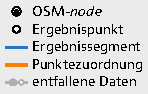
\includegraphics{../chapter6/legend-nodematch-gen}}
		\put(168,35){\figuremark{1}}
		\put(161,85){\figuremark{2}}
		\put(107,33){\figuremark{3}}
	\end{overpic}
	% 1:3500 Google Mercator rotated 10°, bbox 771595 6612098 771840 6612238
	\caption{Verbleibende Topologielücken (Subbelrather Straße~/ Innere Kanalstraße, Köln)}
	\label{fig:kanal-gen-cleanup}
}{
	\begin{overpic}[width=\ScaleIfNeeded]{../chapter6/roundabout-gen-cleanup}
		\put(0,0){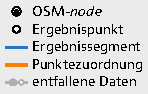
\includegraphics{../chapter6/legend-nodematch-gen}}
	\end{overpic}
	% 1:2000 Google Mercator, bbox 785968 6600972 786108 6601052
	\caption{Verhalten am Kreisverkehr (Friedrichstraße, Köln-Porz)}
	\label{fig:roundabout-gen-cleanup}
}

Das in Abschnitt~\ref{ch:relocateGeneralisedNodes} beschriebene Verfahren funktioniert nicht in jeder Situation, wie Abbildung~\ref{fig:kanal-gen-cleanup} zeigt.
Zwar führt es zu einem gelungenen Ergebnis bei \textfiguremark{1}.
Bei \textfiguremark{2} wird hingegen aufgrund der spezifischen Kreuzungsgeometrie kein „geeigneter“ Punkt auf einer der generalisierten Linien gefunden.
Die dortige Lücke in der Topologie bleibt somit bestehen.
Schließlich kommt bei \textfiguremark{3} das Verfahren zur Lückenbeseitigung gar nicht erst zur Anwendung, weil hier durch den sehr spitzen Winkel der Abbiegefahrbahn mehr als zwei parallele Linienzüge erkannt und generalisiert werden und infolgedessen kein Endpunkt eines \emph{nicht} generalisierten Linienzugs existiert, der zur Lückenbeseitigung verschoben werden könnte (zur Generalisierung mehrerer Parallelen siehe Abschnitt~\ref{ch:iterated-execution} unten).
Ähnliche Probleme existieren an vielen innerstädtischen Kreuzungen mit ungewöhnlicher Geometrie.

Zwar ließe sich argumentieren, dass in vielen dieser Fälle die Attribute der \osm-Daten fehlerhaft sind.
Beispielsweise sollte in Abbildung~\ref{fig:kanal-gen-cleanup} die \textfiguremark{1} und \textfiguremark{3} verbindende Abbiegefahrbahn eigentlich als solche klassifiziert werden (\osmtag{highway}[primary\_link] statt \term{primary}), wodurch vermieden würde, dass sie bei \textfiguremark{3} als parallel zur Hauptfahrbahn erkannt wird. \cf{osm:HighwayLink}

Allerdings ist gerade dieser Fehler im NRW-Testdatensatz sehr stark verbreitet.
So sind in der Kölner Innenstadt (bis einschließlich der Ringe) von insgesamt 79
% 6+13+15+11+26+8
Abbiegefahrbahnen ganze 26
% 2+3+6+5+9+1
nicht als solche klassifiziert.
Es ist auch fraglich, ob hier mit fortschreitender Bearbeitung der \osm-Datenbank Verbesserungen zu erwarten sind, denn Abbiegefahrbahnen und Hauptfahrbahnen werden auf \href{https://www.openstreetmap.org/}{\nolinkurl{osm.org}} mit der gleichen Linearsignatur gezeichnet, so dass eine falsche Klassifizierung beim Betrachten nicht auffällt.
% gemeint ist der Effekt, dass crowdgesourcte VGI im Laufe der Zeit zu Korrektheit tendiert
Vor dem Hintergrund der Aufgabenstellung, die das Ziel \emph{praxistauglicher} Algorithmen vorgibt, ist folglich offensichtlich, dass dieses Problem einer automatisierten Lösung bedarf.

An Kreisverkehren gibt es ebenfalls typische Probleme.
Abbildung~\ref{fig:roundabout-gen-cleanup} zeigt, wie alle im Kreis einander gegenüberliegenden Segmente als parallel erkannt werden.
Mit dieser Masse widersprüchlicher Punktezuordnungen kann der Algorithmus zur Zusammenfassung keine brauchbaren Ergebnisse mehr liefern.
Auch der in Abschnitt~\ref{ch:relocateGeneralisedNodes} besprochene Ansatz zur Beseitigung von Lücken in der Topologie läuft ins Leere.

Zwar ließen sich die meisten Kreisverkehre über \osm-\term{tags} erkennen und von der Generalisierung ausschließen (aus Zeitgründen nicht mehr als Teil dieser Arbeit umgesetzt).
Eine Generalisierung der Kreisverkehre -- zum~Beispiel durch Qualitätsumschlag der linearen Kreisfahrbahn in einen einzelnen Kreuzungspunkt -- könnte jedoch überaus nützlich sein, etwa bei der Herstellung einer Straßenkarte im mittleren Maßstabsbereich.

Auffallend ist, dass alle diskutierten Probleme an Kreuzungen auftreten.
Auf freier Strecke funktioniert die entwickelte Software weitgehend problemlos.
Gäbe es eine zuverlässige Methode, automatisiert Kreuzungen zu erkennen, ließe sich möglicherweise leicht Praxistauglichkeit erzielen.

%Abbildung XY zeigt weitere Beispiele des Scheiterns an unterschiedlichen Kreuzungen.

\begin{itemize}
\item umfangreiche Problemdarstellung verschiedener Typen von Kreuzungen
\end{itemize}



\section{Effizienz}

...



\section{Wiederholtes Ausführen für mehr als zwei Parallele}
\label{ch:iterated-execution}

...



\section{Anwendung auf andere Spezialfälle}

...



% single-chapter commands
%\onlyinsubfile{\listoffigures}
%\onlyinsubfile{\listoftables}
%\onlyinsubfile{% global bibliography settings

\nocite{*}  % include works in bibliography that aren't cited anywhere in the document (for debugging)

\setbibpreamble{Die Literaturangaben sind alphabetisch nach den Nachnamen der Autoren sortiert. Bei mehreren Autoren wird nach dem ersten Autor sortiert.\par\bigskip\bigskip}

\bibliography{../references-papers,../references-manual}
%\bibliography{../references-manual}
}
\end{document}
